\chapter*{Liste des Sigles et Acronymes}
\addcontentsline{toc}{chapter}{Liste des Sigles et Acronymes}

Chaque sigle est accompagné de sa signification officielle et d'une \textbf{définition simple} (« ce qu'il faut savoir dire en une phrase » à l'écrit comme à l'oral).

\section*{1. SRM Souss-Massa, Droit et Secteur Eau-Électricité}

{\small
\begin{longtable}{|p{1.9cm}|p{4.9cm}|p{8.7cm}|}
\hline
\rowcolor{gray!20} \textbf{Sigle} & \textbf{Signification} & \textbf{Définition simple} \\ \hline
\endfirsthead
\hline
\rowcolor{gray!20} \textbf{Sigle} & \textbf{Signification} & \textbf{Définition simple} \\ \hline
\endhead
\textbf{SRM} & Société Régionale Multiservices & Société anonyme à capitaux publics gérant, par région, la distribution d'eau, d'électricité, l'assainissement liquide et l'éclairage public (loi 83-21). \\ \hline
\textbf{RAMSA} & Régie Autonome Multi-Services d'Agadir & Ancienne régie municipale d'Agadir, remplacée par la SRM Souss-Massa le 15 octobre 2024. \\ \hline
\textbf{ONEE} & Office National de l'Électricité et de l'Eau potable & Opérateur national historique, producteur d'électricité et d'eau potable en gros, partenaire des SRM. \\ \hline
\textbf{RADEEMA / RADEEF} & Régies Autonomes de Distribution d'Eau et d'Électricité (Marrakech / Fès) & Anciennes régies municipales comparables à la RAMSA, elles aussi appelées à être remplacées par les SRM régionales. \\ \hline
\textbf{Lydec / Amendis} & Concessionnaires privés historiques (Casablanca / Tanger-Tétouan) & Opérateurs privés de distribution d'eau et d'électricité, également concernés par la réforme des SRM. \\ \hline
\textbf{BO} & Bulletin Officiel & Publication officielle des lois marocaines ; la loi 83-21 est publiée au BO n° 7213 du 17 juillet 2023. \\ \hline
\textbf{SA} & Société Anonyme & Forme juridique de la SRM Souss-Massa, à capitaux 100 \% publics (État, Région, communes). \\ \hline
\textbf{DGSSI} & Direction Générale de la Sécurité des Systèmes d'Information & Autorité nationale de cybersécurité (loi 05-20), pertinente pour la protection des systèmes de supervision des réseaux d'eau/électricité. \\ \hline
\textbf{SCADA} & \textit{Supervisory Control And Data Acquisition} & Système de supervision et de contrôle à distance d'installations industrielles (réseaux d'eau/électricité) ; notion de contexte, non confirmée comme testée à cet examen. \\ \hline
\end{longtable}
}

\section*{2. Informatique, Réseaux et Cybersécurité (Épreuve de Spécialité)}

{\small
\begin{longtable}{|p{1.9cm}|p{4.9cm}|p{8.7cm}|}
\hline
\rowcolor{gray!20} \textbf{Sigle} & \textbf{Signification} & \textbf{Définition simple} \\ \hline
\endfirsthead
\hline
\rowcolor{gray!20} \textbf{Sigle} & \textbf{Signification} & \textbf{Définition simple} \\ \hline
\endhead
\textbf{OSI} & \textit{Open Systems Interconnection} & Modèle de référence en 7 couches qui décrit comment les données circulent dans un réseau. \\ \hline
\textbf{TCP / UDP / IP} & \textit{Transmission Control Protocol / User Datagram Protocol / Internet Protocol} & TCP : transport fiable avec connexion ; UDP : transport rapide sans garantie ; IP : adressage et acheminement des paquets. \\ \hline
\textbf{VLAN} & \textit{Virtual Local Area Network} & Découpage logique d'un réseau physique en réseaux isolés (ex. un VLAN par service technique). \\ \hline
\textbf{VPN} & \textit{Virtual Private Network} & Tunnel chiffré reliant un site distant au réseau central via Internet (IPsec, SSL/TLS). \\ \hline
\textbf{NAT / PAT} & \textit{Network / Port Address Translation} & Traduction des adresses privées en adresse publique pour accéder à Internet. \\ \hline
\textbf{DHCP / DNS} & \textit{Dynamic Host Configuration Protocol / Domain Name System} & Attribution automatique des adresses IP / traduction des noms de domaine en adresses IP. \\ \hline
\textbf{OSPF / BGP} & \textit{Open Shortest Path First / Border Gateway Protocol} & Protocoles de routage dynamique : OSPF à l'intérieur d'une organisation, BGP entre opérateurs sur Internet. \\ \hline
\textbf{MPLS} & \textit{Multiprotocol Label Switching} & Technologie opérateur qui achemine le trafic par étiquettes ; base des réseaux privés d'entreprise (WAN). \\ \hline
\textbf{WAN / LAN / WLAN} & \textit{Wide / Local / Wireless Local Area Network} & Réseau étendu (entre sites) / réseau local / réseau local sans fil (Wi-Fi). \\ \hline
\textbf{QoS} & \textit{Quality of Service} & Priorisation de certains flux (voix, supervision temps réel) sur le réseau. \\ \hline
\textbf{VoIP / SIP} & \textit{Voice over IP / Session Initiation Protocol} & Téléphonie sur le réseau informatique ; SIP établit les appels. \\ \hline
\textbf{FTTH / FTTO} & \textit{Fiber To The Home / Office} & Fibre optique jusqu'au domicile / jusqu'au bureau. \\ \hline
\textbf{PKI} & \textit{Public Key Infrastructure} & Infrastructure de gestion des certificats numériques (identités, signature, chiffrement). \\ \hline
\textbf{TLS / HTTPS} & \textit{Transport Layer Security} & Chiffrement des échanges web ; HTTPS = HTTP sécurisé par TLS (port 443). \\ \hline
\textbf{IDS / IPS} & \textit{Intrusion Detection / Prevention System} & Détection / blocage des intrusions sur le réseau. \\ \hline
\textbf{SIEM / SOC} & \textit{Security Information and Event Management / Security Operations Center} & Outil de centralisation des journaux / équipe de surveillance de la sécurité en continu. \\ \hline
\textbf{MFA} & \textit{Multi-Factor Authentication} & Authentification à plusieurs facteurs (mot de passe + téléphone ou carte). \\ \hline
\textbf{CNDP} & Commission Nationale de contrôle de la protection des Données à caractère Personnel & Autorité de la loi 09-08 sur les données personnelles (données des abonnés eau/électricité). \\ \hline
\textbf{ISO 27001} & Norme internationale de management de la sécurité de l'information & Référentiel du SMSI (analyse des risques, mesures, amélioration continue). \\ \hline
\textbf{PRA / PCA} & Plan de Reprise / de Continuité d'Activité & Redémarrer après un sinistre / continuer à fonctionner pendant l'incident (indicateurs RTO et RPO). \\ \hline
\textbf{RAID} & \textit{Redundant Array of Independent Disks} & Regroupement de disques pour la performance ou la tolérance aux pannes (RAID 1 miroir, RAID 5 parité). \\ \hline
\textbf{SLA} & \textit{Service Level Agreement} & Engagement chiffré de niveau de service (disponibilité, délais). \\ \hline
\textbf{POO} & Programmation Orientée Objet & Paradigme fondé sur les classes et objets (encapsulation, héritage, polymorphisme). \\ \hline
\textbf{UML} & \textit{Unified Modeling Language} & Langage de modélisation graphique des logiciels (cas d'utilisation, classes, séquence). \\ \hline
\textbf{MCD / MLD} & Modèle Conceptuel / Logique de Données (Merise) & Schéma entités-associations / traduction en tables relationnelles. \\ \hline
\textbf{SQL} & \textit{Structured Query Language} & Langage des bases de données relationnelles. \\ \hline
\textbf{ACID} & Atomicité, Cohérence, Isolation, Durabilité & Les quatre garanties d'une transaction fiable. \\ \hline
\textbf{API / REST} & \textit{Application Programming Interface / Representational State Transfer} & Interface permettant à deux logiciels de communiquer ; REST = style d'API web sans état sur HTTP. \\ \hline
\textbf{MVC} & Modèle-Vue-Contrôleur & Architecture qui sépare données, affichage et logique. \\ \hline
\textbf{CI/CD} & \textit{Continuous Integration / Continuous Delivery} & Automatisation des tests et des déploiements. \\ \hline
\textbf{IaaS / PaaS / SaaS} & \textit{Infrastructure / Platform / Software as a Service} & Trois niveaux de service du cloud. \\ \hline
\textbf{OWASP} & \textit{Open Web Application Security Project} & Référentiel des dix principaux risques de sécurité des applications web. \\ \hline
\textbf{SGBD} & Système de Gestion de Bases de Données & Logiciel de gestion des bases (Oracle, PostgreSQL, MySQL). \\ \hline
\textbf{SI} & Système d'Information & Ensemble des personnes, données, logiciels, matériels et procédures qui traitent l'information d'une organisation. \\ \hline
\textbf{SIG} & Système d'Information Géographique & Outil de cartographie et de gestion du patrimoine des réseaux d'eau et d'électricité. \\ \hline
\textbf{ETL} & \textit{Extract, Transform, Load} & Processus d'alimentation d'un entrepôt de données à partir de sources multiples (facturation, télérelève, SIG). \\ \hline
\end{longtable}
}

\IfFileExists{images/img_011_def_modele_osi_tcpip.png}{%
\begin{figure}[H]
    \centering
    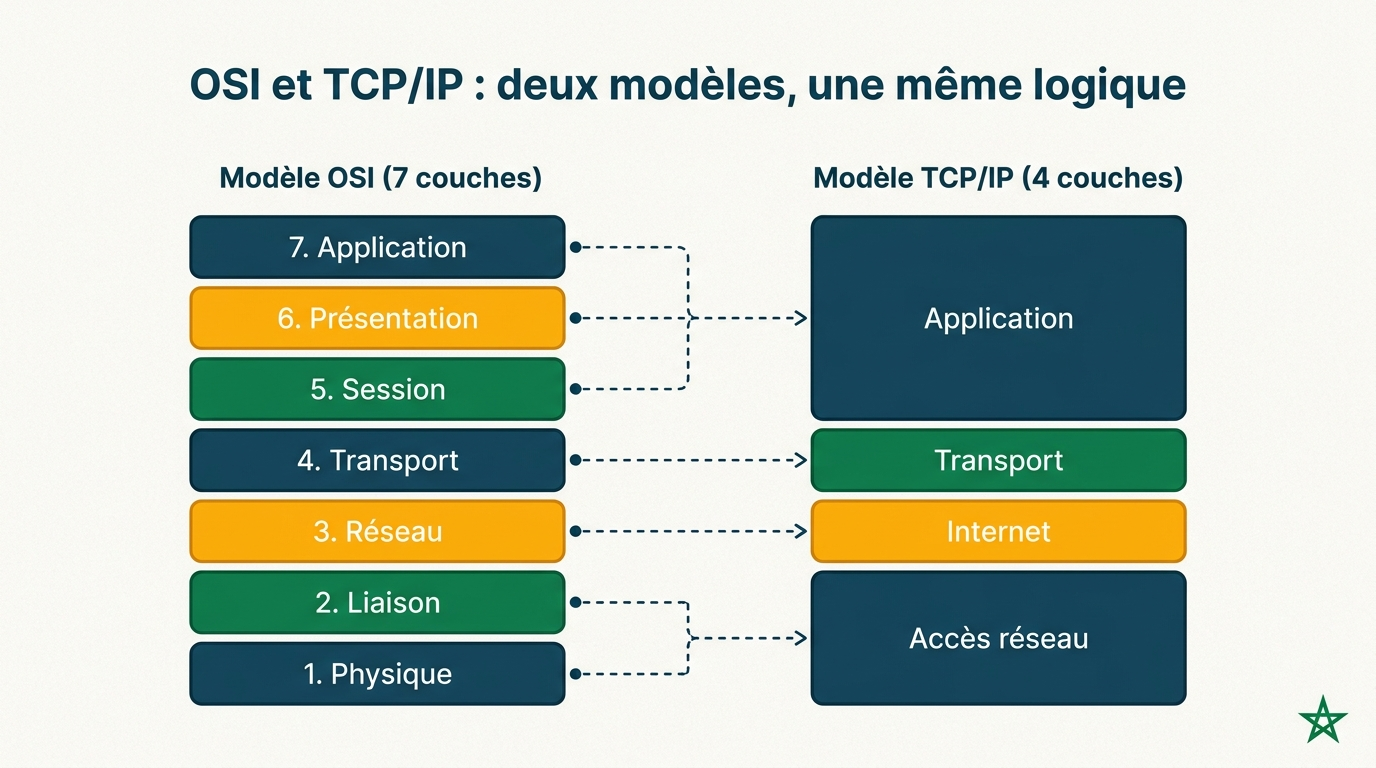
\includegraphics[width=\textwidth]{images/img_011_def_modele_osi_tcpip.png}
    \caption{OSI et TCP/IP : deux modèles, une même logique}
\end{figure}}{}
